%% 06_5-Recipes_IFU.tex
%% Created:     Fri Aug 25 13:14:02 2017 by Koehler@I-Mac
%%
%% subsection for IFU recipes
%%
%%%%%%%%%%%%%%%%%%%%%%%%%%%%%%%%%%%%%%%%%%%%%%%%%%%%%%%%%%%%%%%%%%%%%%%%%%%%%%%

\clearpage
\subsection{LM integral-field spectroscopy (IFU)}
\label{ssec:IFU_recipes}

\TODO{This section is identical to the PDR document \cite{DRLS}. We
will consider rearranging the recipes to be in line with the imaging
pipelines. This would entail handling basic reduction and background
subtraction for both science and standard exposures in common
recipes (\CODE{metis_ifu_basic}, \CODE{metis_ifu_background}), then
having a recipe to analyse the standard observations
(\CODE{metis_ifu_photstd}). The science exposures are then fully
calibrated (\CODE{metis_ifu_calibrate}). A full set of exposures would
then be assembled and restored with a fully sampled PSF in a
post-processing recipe (\CODE{metis_ifu_combine}).}

\subsubsection{IFU wavelength calibration}
\label{sssec:ifu_wavecal}
\label{rec:metis_ifu_wavecal}

This recipe processes daytime wavelength calibration images to derive
the pixel-to-wavelength relation for the LM integral-field
spectrograph. The calibration template will use the \ac{QCL} in the warm calibration unit to finely sample the desired
wavelength range. The image will consist of lines for each wavelength
and slice. The solution will have to provide for each detector pixel
$(x,y)$ the slice number $i$, the spatial position $\xi$ along the
slice and the wavelength in the dispersion correction. As the slices
and wavelength lines may be tilted with respect to the detector
columns and rows, a combined solution is required
\begin{eqnarray}
  \label{eq:wavelength_solution}
  \xi &= f_{i}(x, y) \\
  \lambda &= g_{i}(x, y)
\end{eqnarray}
The boundaries of the slice image on the detector are obtained by
measuring the left and right edges of the wavelength lines and
interpolating. The slice number is then obtained by counting the
slices according to the optical design of the spectrograph. The
wavelength of each line is known from the settings of the \ac{QCL}, the $x$
coordinate is obtained by linear interpolation along the line (or
perhaps using the distortion table from \hyperref[rec:metis_ifu_distortion]{\REC{metis_ifu_distortion}} if
necessary). The functions $f_{i}$ and $g_{i}$ are expected to be
sufficiently accurately described by low-order polynomials.

The recipe produces a multi-extension FITS file with an image
extension mapping wavelength across each detector in the array. A
table extension holds the polynomial coefficients.

 This is in compliance with \REQ{METIS-6074}.

\begin{recipedef}
  Name:                & \hyperref[rec:metis_ifu_wavecal]{\REC{metis_ifu_wavecal}}              \\
  Purpose:             & Determine pixel-to-wavelength transformation.                          \\
  Requirements:        & \REQ{METIS-6074}                                                       \\
  Type:                & Calibration                                                            \\
  Templates:           & \TPL{METIS_ifu_cal_InternalWave}                                       \\
  Input data:          & \hyperref[dataitem:ifu_wave_raw]{\RAW{IFU_WAVE_RAW}}           \\
                       & \hyperref[dataitem:master_dark_ifu]{\PROD{MASTER_DARK_IFU}}            \\
                       & \hyperref[dataitem:badpix_map_ifu]{\PROD{BADPIX_MAP_IFU}}              \\
                       & \hyperref[dataitem:ifu_distortion_table]{\PROD{IFU_DISTORTION_TABLE}}   \\
  Parameters:          & None                                                                   \\
  Algorithm:           & Measure line locations (left and right edges, centroid by Gaussian fit)\\
                       & Compute wavelength solution $\xi(x, y, i)$, $\lambda(x, y, i)$         \\
  Output data:         & \hyperref[dataitem:ifu_wavecal]{\PROD{IFU_WAVECAL}}                    \\
  Expected accuracies: & TBD                                                                    \\
  QC1 parameters:      & \QC{QC IFU WAVECAL RMS}                                                \\
                       & \QC{QC IFU WAVECAL NLINES}                                             \\
                       & \QC{QC IFU WAVECAL PEAK CNTS}                                          \\
                       & \QC{QC IFU WAVECAL LINE WIDTH}                                         \\
  \end{recipedef}

\begin{figure}[hb]
  \centering
  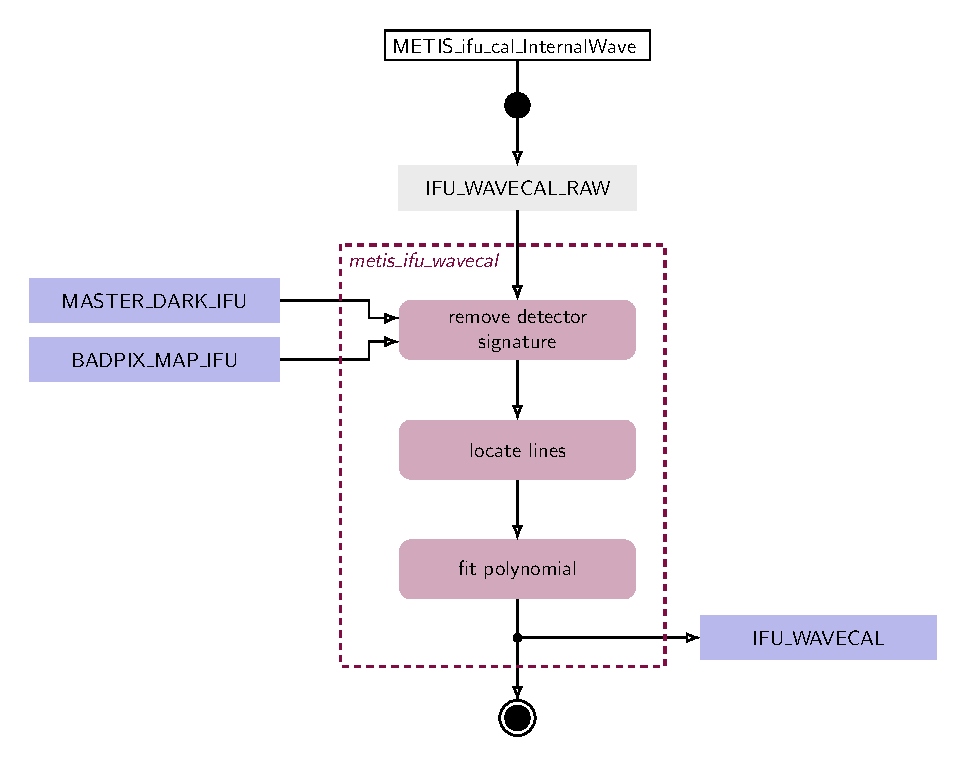
\includegraphics[width=0.7\textwidth]{metis_ifu_wavecal}
  \caption[Recipe: \REC{metis_ifu_wavecal}]{\REC{metis_ifu_wavecal} --
    daytime wavelength calibration for the IFU.}
  \label{fig:metis_ifu_wavecal}
\end{figure}


\clearpage
\subsubsection{IFU relative spectral response function}
\label{sssec:ifu_rsrf}
\label{rec:metis_ifu_rsrf}

This recipe creates a spectroscopic master flat and determines the
relative spectral response function (RSRF) for the four HAWAII2RG
detectors of the LM spectrograph. The input data are obtained by
illuminating the field of view with the black-body calibration lamp at
two different temperatures. The RSRF is then determined by dividing
the image by the known lamp continuum shape for the respective
temperature. We refer to the two-dimensional image obtained by this
division as \hyperref[dataitem:master_flat_ifu]{\PROD{MASTER_FLAT_IFU}} and the one-dimensional reponse
function obtained by averaging at constant wavelength as
\PROD{RSRF}. The bad pixel mask can be updated by identifying pixels
that deviate strongly from their neighbours.

\begin{recipedef}
Name:                & \hyperref[rec:metis_ifu_rsrf]{\REC{metis_ifu_rsrf}}                                                     \\
Purpose:             & Create relative spectral response function for the IFU detector.         \\
Requirements:        & \REQ{METIS-6131}, \REQ{METIS-6698}                                       \\
Type:                & Calibration                                                              \\
Templates:           & \TPL{METIS_ifu_cal_rsrf}                                                 \\
Input data:          & \hyperref[dataitem:ifu_rsrf_raw]{\RAW{IFU_RSRF_RAW}} (Raw flats taken with black-body calibration lamp.)   \\
                     & \hyperref[dataitem:master_dark_ifu]{\PROD{MASTER_DARK_IFU}}              \\
                     & \hyperref[dataitem:badpix_map_ifu]{\PROD{BADPIX_MAP_IFU}}                                                    \\
                     & \hyperref[dataitem:ifu_wavecal]{\PROD{IFU_WAVECAL}}: image with wavelength at each pixel.                 \\
Parameters:          & None                                                                     \\
Algorithm:           & Create continuum image by mapping Planck spectrum at $T_{\mathrm{lamp}}$ to
                       wavelength image.                                                        \\
                     & Divide exposures by continuum image.                                     \\
                     & Average exposures to yield master flat (2D RSRF).                        \\
                     & Average in spatial direction to obtain relative response function        \\
Output data:         & \hyperref[dataitem:master_flat_ifu]{\PROD{MASTER_FLAT_IFU}}                                                   \\
                     & \hyperref[dataitem:rsrf_ifu]{\PROD{RSRF_IFU}}                                                          \\
                     & \hyperref[dataitem:badpix_map_ifu]{\PROD{BADPIX_MAP_IFU}}                                                    \\
Expected accuracies: & TBD                                                                      \\
QC1 parameters:      & \QC{QC IFU RSRF NBADPIX}                                                    \\
                     & (more TBD)                                                               \\
\end{recipedef}

\begin{figure}[hb]
  \centering
  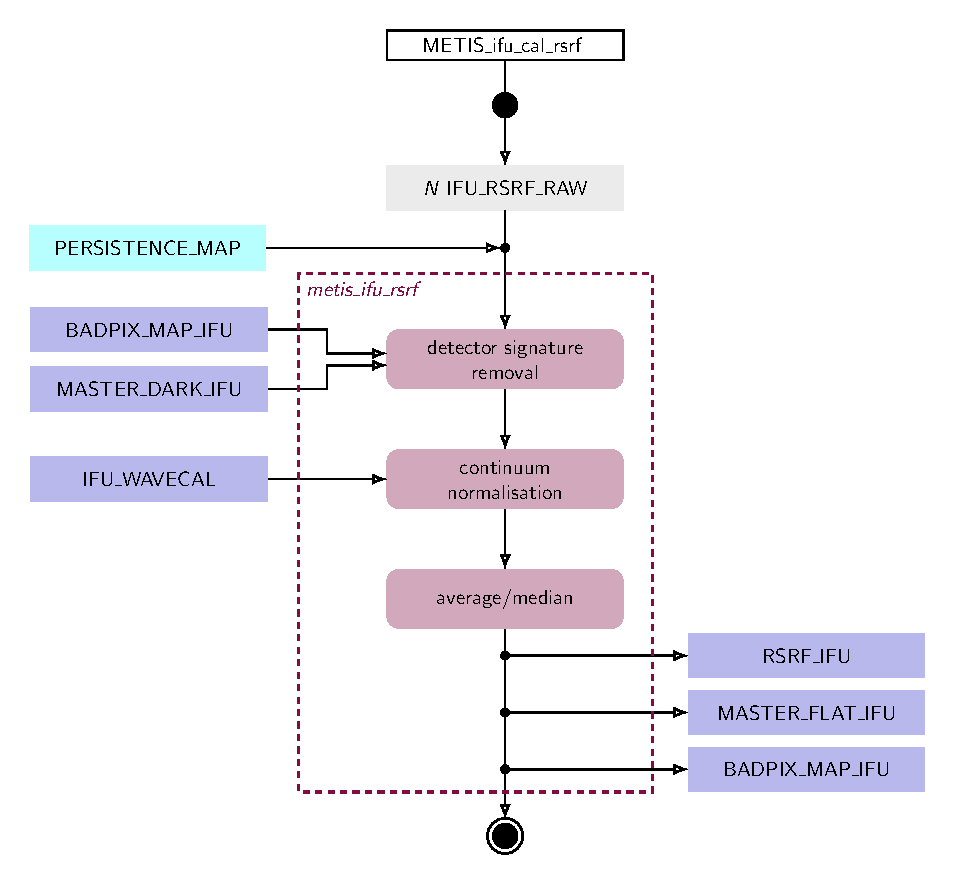
\includegraphics[width=0.6\textwidth]{metis_ifu_rsrf}
  \caption[Recipe: \REC{metis_ifu_rsrf}]{\REC{metis_ifu_rsrf} --
    creation of IFU relative spectral response function.}
  \label{fig:metis_ifu_rsrf}
\end{figure}


\clearpage
\subsubsection{IFU flux standard reduction}
\label{sssec:ifu_std_process}
\label{rec:metis_ifu_std_process}

This recipe reduces and analyses a series of IFU observations of a
spectroscopic flux standard star. The comparison of the measured
detector counts (ADU) with the tabulated spectrum of the star gives
the wavelength-dependent conversion from ADU to physical units
(photons per second per per centimetre square per wavelength bin per
spatial bin).

The level of stray light is estimated in the dark areas between the
spectra and subtracted from the entire frame. The distribution of
stray light across the field can only be characterised once the
instrument is built. It is to be hoped that subtraction of a constant
or a low-level 2D polynomial fit will be sufficient.

The sky and thermal background is estimated from blank sky
observations (if obtained during the observing sequence) or by
combining the (dithered) science frames.

The wavelength calibration is taken from the daylight calibration. It
may be refined by measuring telluric emission and/or absorption lines
(by fitting with \lstinline{molecfit}).

\begin{recipedef}
  Name:                & \hyperref[rec:metis_ifu_std_process]{\REC{metis_ifu_std_process}}                                            \\
  Purpose:             & Determine conversion between detector counts and physical source flux. \\
  Requirements:        & \REQ{METIS-6131}                                                       \\
  Type:                & Calibration                                                            \\
  Templates:           & \TPL{METIS_ifu_cal_standard}                                           \\
  Input data:          & \hyperref[dataitem:ifu_std_raw]{\RAW{IFU_STD_RAW}} (Raw spectra of flux standard star)                  \\
                       & \hyperref[dataitem:master_dark_ifu]{\PROD{MASTER_DARK_IFU}}            \\
                       & \hyperref[dataitem:rsrf_ifu]{\PROD{RSRF_IFU}} (2D relative spectral response function)               \\
                       & \hyperref[dataitem:badpix_map_ifu]{\PROD{BADPIX_MAP_IFU}}  \\
                       & \hyperref[dataitem:ifu_wavecal]{\PROD{IFU_WAVECAL}} \\
                       & \hyperref[dataitem:ifu_distortion_table]{\PROD{IFU_DISTORTION_TABLE}} \\
  Parameters:          & None                                                                   \\
  Algorithm:           & Subtract dark, divide by master flat                                   \\
                       & Estimate stray light and subtract                                      \\
                       & Estimate background and subtract                                       \\
                       & Rectify spectra and assemble cube                                      \\
                       & Extract 1D spectrum of star                                            \\
                       & Compute and apply telluric correction                                  \\
                       & Compute conversion to physical units as function of wavelength.        \\
  Output data:         & \hyperref[dataitem:ifu_std_reduced_cube]{\PROD{IFU_STD_REDUCED_CUBE}}  \\
                       & \hyperref[dataitem:ifu_std_background_cube]{\PROD{IFU_STD_BACKGROUND_CUBE}}                                         \\
                       & \hyperref[dataitem:ifu_std_reduced_1d]{\PROD{IFU_STD_REDUCED_1D}}                                              \\
                       & \hyperref[dataitem:ifu_std_telluric_1d]{\PROD{IFU_STD_TELLURIC_1D}}                                             \\
                       & \hyperref[dataitem:fluxcal_tab]{\PROD{FLUXCAL_TAB}}                                                     \\
  Expected accuracies: & TBD                                                                    \\
  QC1 parameters:      & \QC{QC IFU STD STRAYLIGHT MEAN}                                        \\
\end{recipedef}

\begin{figure}[hb]
  \centering
  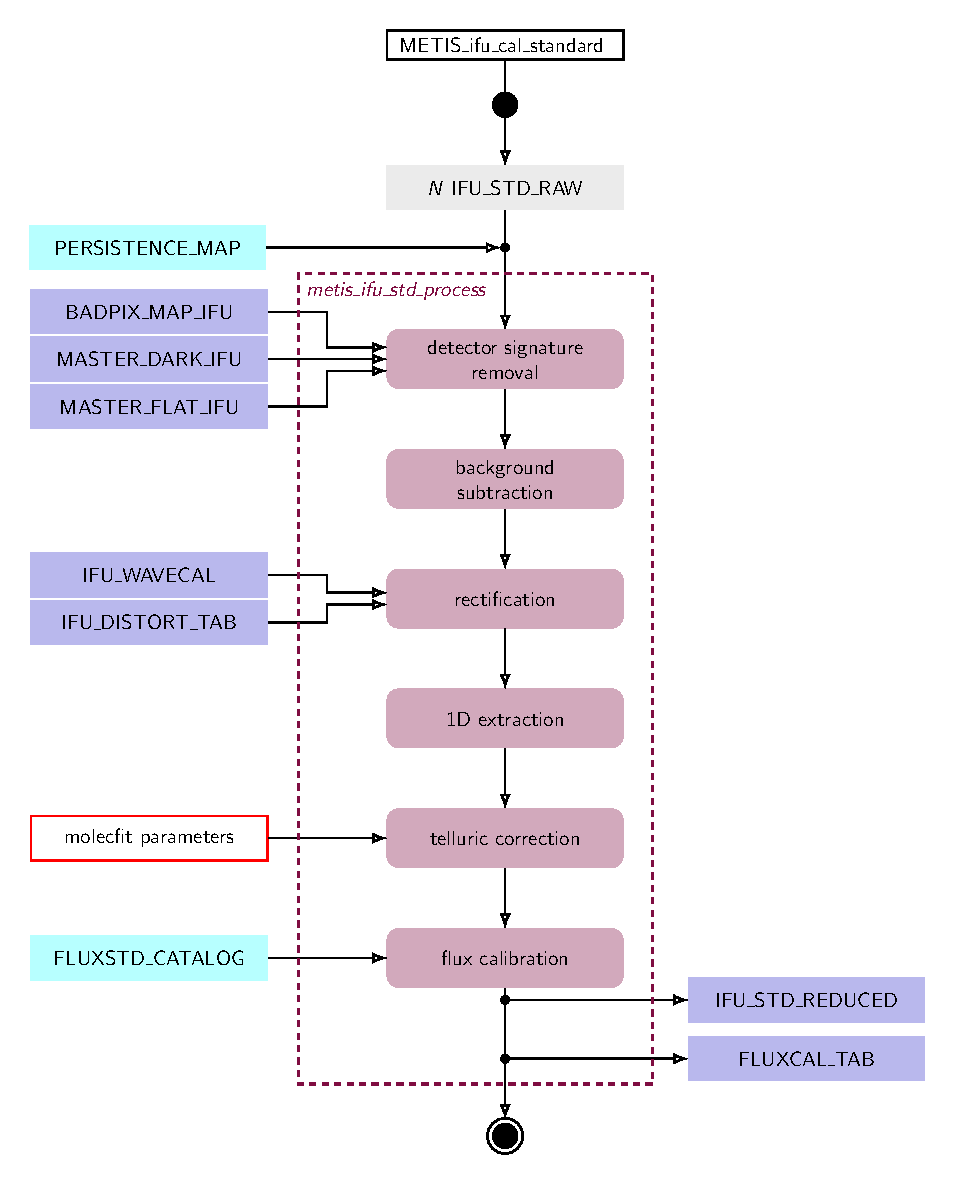
\includegraphics[width=0.7\textwidth]{metis_ifu_std_process}
  \caption[Recipe: \REC{metis_ifu_std_process}]{%
    \hyperref[rec:metis_ifu_std_process]{\REC{metis_ifu_std_process}} -- reduction of IFU flux standard
    frames and flux calibration (not all data products are shown).}
  \label{fig:metis_ifu_std_process}
\end{figure}

\clearpage
\subsubsection{IFU science reduction}
\label{sssec:ifu_sci_process}
\label{rec:metis_ifu_sci_process}

This recipe performs basic reduction of raw science exposures applying
dark and RSRF correction and flux calibration (i.e.~conversion of
pixel values to physical units) on each exposure individually. The
recipe shall be able to process data from either the nominal or the
extended wavelength mode. For the nominal mode, all slices belong to
the same echelle order. For the extended mode, slices belonging to the
same echelle order are grouped and processing is iterated over the
echelle orders.

The level of stray light is estimated in the dark areas between the
spectra and subtracted from the entire frame. The distribution of
stray light across the field can only be characterised once the
instrument is built. It is to be hoped that subtraction of a constant
or a low-level 2D polynomial fit will be sufficient.

The sky and thermal background, as well as residual straylight, is
estimated from blank sky observations if these are available in the
sequence of input frames or by combining (dithered) science
frames. The initial wavelength solution is taken from the daylight
calibration. It may be checked and corrected by measuring atmospheric
lines if a sufficient number is available in the limited wavelength
range.

A telluric correction is determined by this recipe by automatically
extracting a 1D spectrum from ``object'' pixels identified by a
thresholding algorithm. \lstinline{molecfit} is applied to this
spectrum and the correction is mapped back to the reduced 2D images or
3D cubes using the wavelength images. In an interactive environment
(Reflex workflow) the telluric correction may be improved by asking
the user to define an extraction aperture adapted to the target
structure.

Various levels of output data can be envisaged:
\begin{itemize}
\item Reduced 2D detector images. These are accompanied by additional
  information describing the geometry of the slice layout, target
  position and wavelength calibration to the extent that the exposure can be
  combined with other exposures into a single rectified spectral cube.
  This information can be stored in the FITS header or a table
  extension.
\item A rectified spectral cube for each exposure with a linear
  wavelength grid, constructed by resampling each spectral slice onto
  a spatial-wavelength grid common to all slices. The spatial pixels
  are rectangular with along-slit pixel scale given by the detector
  pixel scale and the across-slit pixel scale given by the slice
  width.
\item A spectral cube obtained by combining all exposures taken within
  a template. This step involves the image reconstruction discussed in
  Sect.~8.9 of \cite{DRLS}. Whether this step is included
  in the present recipe \hyperref[rec:metis_ifu_sci_process]{\REC{metis_ifu_sci_process}} or is postponed to
  the more general recipe \hyperref[rec:metis_ifu_sci_postprocess]{\REC{metis_ifu_sci_postprocess}} is TBD. It
  may be formally required to do the image reconstruction here if
  templates are set up to obtain a fixed set of spatially dithered and
  rotated exposures aimed at reconstructing a fully sampled PSF in
  both spatial dimensions.
\end{itemize}

For the nominal mode, each output is a single-extension FITS file
corresponding to one echelle order. For the extended mode, each of the
echelle orders results in an extension in a multi-extension FITS
file.

The recipe as described here is run in the science pipelines. For the
observatory pipeline, a variant of the recipe may be implemented with
reduced functionality and output. The observatory recipe may also have
to include features to determine QC parameters for the LM-band images
that are taken in parallel with the IFU exposures, similar to
 \hyperref[rec:metis_lm_img_basic_reduce]{\REC{metis_lm_img_basic_reduce}}.

\begin{recipedef}
Name:                & \hyperref[rec:metis_ifu_sci_process]{\REC{metis_ifu_sci_process}}                                                              \\
Purpose:             & Reduction of individual science exposures.                                               \\
Requirements:        & \REQ{METIS-6131}                                                                         \\
Type:                & Science                                                                                  \\
Templates:           & \TPL{METIS_ifu_obs_FixedSkyOffset}                                                       \\
                     & \TPL{METIS_ifu_obs_GenericOffset}                                                        \\
                     & \TPL{METIS_ifu_ext_obs_FixedSkyOffset}                                                   \\
                     & \TPL{METIS_ifu_ext_obs_GenericOffset}                                                    \\
% TODO: Decide what to do about app
%                     & \TPL{METIS_ifu_app_obs_GenericOffset}                                                    \\
                     & \TPL{METIS_ifu_vc_obs_FixedSkyOffset}                                                    \\
%                     & \TPL{METIS_ifu_ext_app_obs_GenericOffset}                                                \\
                     & \TPL{METIS_ifu_ext_vc_obs_FixedSkyOffset}                                                \\
% HB 20230626: Not sure the *_obs_Stare templates should go here, but seems the most logical place.
                     & \TPL{METIS_ifu_app_obs_Stare}                                                            \\
                     & \TPL{METIS_ifu_ext_app_obs_Stare}                                                        \\
                     & \TPL{METIS_ifu_cal_psf}                                                                  \\
Input data:          & \hyperref[dataitem:ifu_sci_raw]{\RAW{IFU_SCI_RAW}} (Dithered science exposures.) \\
                     & \hyperref[dataitem:ifu_sky_raw]{\RAW{IFU_SKY_RAW}} (Blank sky images, if available.) \\
                     & \hyperref[dataitem:master_dark_ifu]{\PROD{MASTER_DARK_IFU}}                              \\
                       & \hyperref[dataitem:rsrf_ifu]{\PROD{RSRF_IFU}} (2D relative spectral response function)               \\
                       & \hyperref[dataitem:badpix_map_ifu]{\PROD{BADPIX_MAP_IFU}}  \\
                       & \hyperref[dataitem:ifu_wavecal]{\PROD{IFU_WAVECAL}} \\
% TODO: I believe this should not be just FLUXCAL_TAB as it is not a table but an image
                     & \hyperref[dataitem:fluxcal_tab]{\PROD{FLUXCAL_TAB}} (Flux calibration table) \\
                       & \hyperref[dataitem:ifu_distortion_table]{\PROD{IFU_DISTORTION_TABLE}} \\
                     & \hyperref[dataitem:lsf_kernel]{\STATCALIB{LSF_KERNEL}} (Line spread kernel to be used with \CODE{molecfit}) \\
Parameters:          & telluric correction (yes/no)                                                             \\
                     & more TBD                                                                                 \\
Algorithm:           & Subtract dark, divide by master flat                                                     \\
                     & Estimate stray light and subtract                                                        \\
                     & Estimate background from dithered science exposures or blank-sky exposures and subtract. \\
                     & Apply flux calibration.                                                                  \\
                     & Rectify spectra and assemble cube                                                        \\
                     & Extract 1D object spectrum                                                               \\
                     & Compute telluric correction and apply to reduced images and cube                         \\
Output data:         & \hyperref[dataitem:ifu_sci_reduced]{\PROD{IFU_SCI_REDUCED}} (2D, per exposure)           \\
                     & \hyperref[dataitem:ifu_sci_reduced_tac]{\PROD{IFU_SCI_REDUCED_TAC}} (2D, per exposure)   \\
                     & \hyperref[dataitem:ifu_sci_background]{\PROD{IFU_SCI_BACKGROUND}} (2D, per exposure)     \\
                     & \hyperref[dataitem:ifu_sci_reduced_cube]{\PROD{IFU_SCI_REDUCED_CUBE}} (3D, per exposure) \\
                     & \hyperref[dataitem:ifu_sci_reduced_cube_tac]{\PROD{IFU_SCI_REDUCED_CUBE_TAC}} (3D, per exposure) \\
                     & \hyperref[dataitem:ifu_sci_combined]{\PROD{IFU_SCI_COMBINED}} (3D)                       \\
                     & \hyperref[dataitem:ifu_sci_combined_tac]{\PROD{IFU_SCI_COMBINED_TAC}} (3D)               \\
                     & \hyperref[dataitem:ifu_sci_object_1d]{\PROD{IFU_SCI_OBJECT_1D}}  (1D)                    \\
                     & \hyperref[dataitem:ifu_sci_telluric_1d]{\PROD{IFU_SCI_TELLURIC_1D}}                      \\
Expected accuracies: & TBD                                                                                      \\
QC1 parameters:      & TBD                                                                                      \\
\end{recipedef}

\begin{figure}[hb]
  \centering
  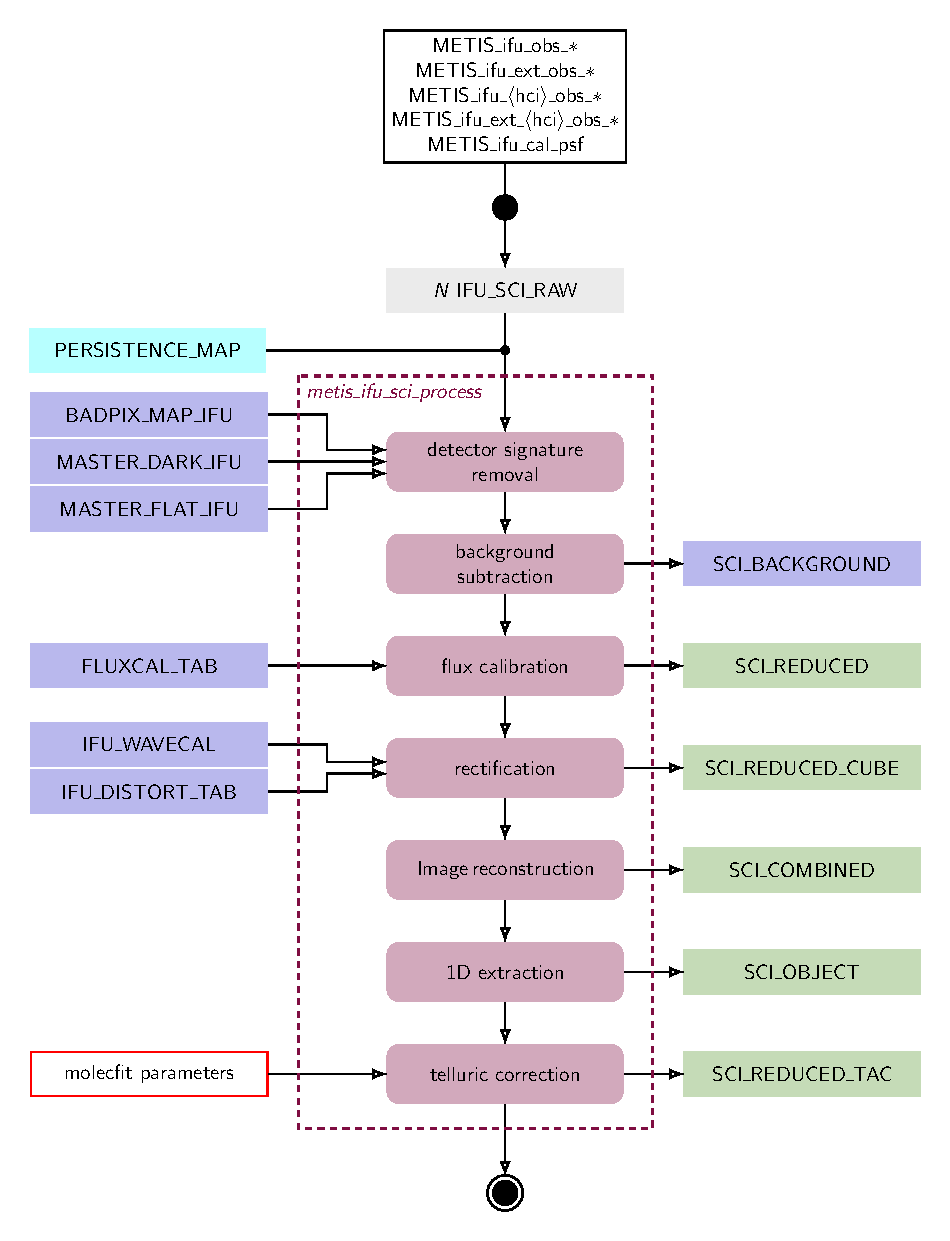
\includegraphics[width=0.7\textwidth]{metis_ifu_sci_process}
  \caption[Recipe: \REC{metis_ifu_sci_process}]{%
    \hyperref[rec:metis_ifu_sci_process]{\REC{metis_ifu_sci_process}} -- reduction of IFU science frames.}
  \label{fig:metis_ifu_sci_process}
\end{figure}



\clearpage
\subsubsection{IFU telluric absorption correction}
\label{sssec:ifu_tellcorr}
\label{rec:metis_ifu_tellcorr}

This recipe corrects for telluric absorption in a reduced IFU data
cube. The correction is done via a model atmospheric spectrum derived
with \CODE{molecfit}.

An automatic telluric correction can be performed as part of
\REC{metis_ifu_sci_process}. In an interactive environment it may be
better to do the telluric correction as a separate post-processing
step with a user-defined aperture for the extraction of a 1D object
spectrum. The spectrum is extracted from a combined cube
(\PROD{IFU_SCI_COMBINED}) but may be applied to other products of
\REC{metis_ifu_sci_process} specified in the input set of frames.

\begin{recipedef}
  Name:                & \hyperref[rec:metis_ifu_tellcorr]{\REC{metis_ifu_tellcorr}}                                                        \\
  Purpose:             & Remove telluric absorption features                                             \\
  Requirements:        & \REQ{METIS-6091}                                                                \\
  Type:                & Calibration / post processing                                                   \\
  Templates:           & ---                                                                             \\
  Input data:          & \hyperref[dataitem:ifu_sci_combined]{\PROD{IFU_SCI_COMBINED}} -- reduced combined IFU cube                            \\
                       & \hyperref[dataitem:lsf_kernel]{\STATCALIB{LSF_KERNEL}} -- Line spread kernel to be used with \CODE{molecfit}         \\
                       & \hyperref[dataitem:atm_profile]{\EXTCALIB{ATM_PROFILE}} -- Atmospheric input profile to be used with \CODE{molecfit} \\
  Parameters:          & extraction aperture parameters                                                  \\
                       & \CODE{molecfit} parameters                                                      \\
                       & atmospheric profile incl.\ radiometer data                                      \\
                       & line spread kernel                                                              \\
  Algorithm:           & extract 1D spectrum                                                             \\
                       & Application of molecfit                                                         \\
  Output data:         & \hyperref[dataitem:ifu_sci_reduced_tac]{\PROD{IFU_SCI_REDUCED_TAC}}                                                      \\
  Expected accuracies: & TBD                                                                             \\
  QC1 parameters:      & TBD                                                                             \\
\end{recipedef}

\begin{figure}[hb]
  \centering
  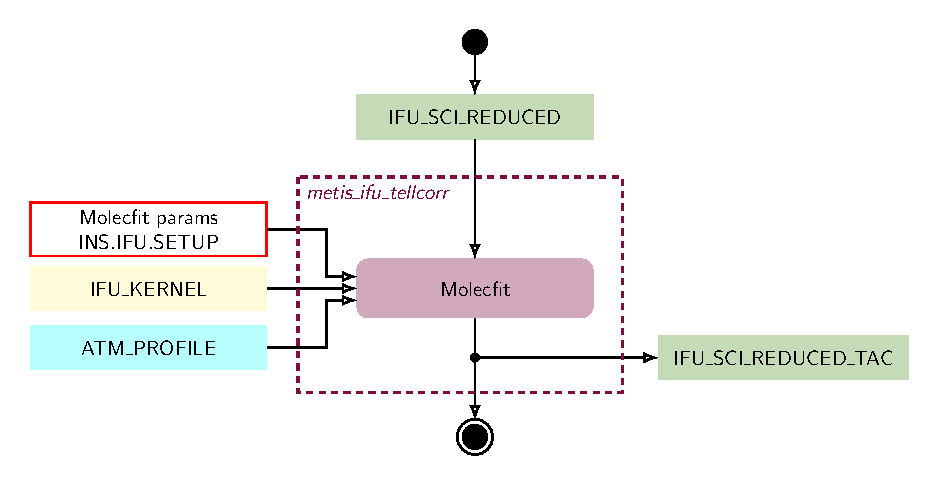
\includegraphics[width=0.7\textwidth]{metis_ifu_tellcorr}
  \caption[Recipe: \REC{metis_ifu_tellcorr}]{\REC{metis_ifu_tellcorr}
    -- telluric correction of reduced IFU science cubes.}
  \label{fig:metis_ifu_tellcorr}
\end{figure}


\clearpage
\subsubsection{IFU science postprocessing}
\label{sssec:ifu_sci_postprocess}
\label{rec:metis_ifu_sci_postprocess}

This recipe combines a number of reduced IFU exposures covering a
different spatial and wavelength ranges into a single data cube. The
positions and orientations of the exposures may differ as follows (cf. \cite{METIS-operational_concept}): %\TODO{Reference to operational concept}
\begin{description}
\item[Spatial dithering:] The target is placed at different positions
  along and across the slice. Along-slice dithering aids in background
  subtraction, across-slice dithering is necessary image
  reconstruction given that the slice width undersamples the PSF.
\item[Field rotation:] The field is rotated by 90 degrees between
  exposures. The cube of a single exposure has different pixel scales
  along and across the slice. The goal of combining exposures at
  different rotation angles is to reconstruct images on a square grid
  with pixel scale given by the detector scale (8.2\,mas). The exact
  procedure remains to be investigated; one of the major challenges is
  to find the exact centre of rotation
  (Sect.~8.9 of \cite{DRLS}).
\item[Spectral dithering:] Sequences of exposures are taken at various
  echelle angles in order to cover an increased contiguous wavelength
  range. In the extended mode, such a sequence may cover the
  wavelength gaps between echelle order coverage.
\end{description}

In order to allow co-addition of data from separate OBs, possibly taken
months apart, the wavelengths will be corrected to the heliocentric
reference system before co-addition.

The recipe is only used in the science-grade pipelines, not at the
observatory.

\begin{recipedef}
  Name:           & \hyperref[rec:metis_ifu_sci_postprocess]{\REC{metis_ifu_sci_postprocess}}                                            \\
  Purpose:        & Coaddition and mosaicing of reduced science cubes.                         \\
  Requirements:   & \REQ{METIS-6131}                                                           \\
  Type:           & Science                                                                    \\
  Templates:      & None                                                                       \\
  Input data:     & Reduced science cubes (\hyperref[dataitem:ifu_sci_reduced]{\PROD{IFU_SCI_REDUCED}}, \hyperref[dataitem:ifu_sci_reduced_tac]{\PROD{IFU_SCI_REDUCED_TAC}}) \\
  Parameters:     & TBD                                                                        \\
  Algorithm:      & Determine cubic output grid encompassing all input cubes                   \\
                  & Resample input cubes to output grid                                        \\
                  & Coadd                                                                      \\
  Output data:    & \hyperref[dataitem:ifu_sci_coadd]{\PROD{IFU_SCI_COADD}}                                                       \\
                  & \hyperref[dataitem:ifu_sci_coadd_error]{\PROD{IFU_SCI_COADD_ERROR}}                                                 \\
  QC1 parameters: & ---                                                                        \\
\end{recipedef}

\begin{figure}[hb]
  \centering
  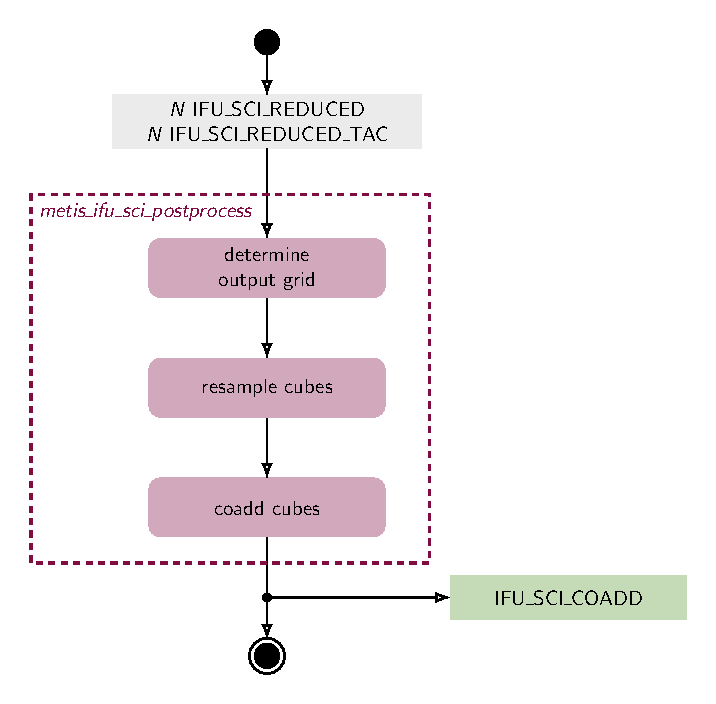
\includegraphics[width=0.7\textwidth]{metis_ifu_sci_postprocess}
  \caption[Recipe: \REC{metis_ifu_sci_postprocess}]{%
    \hyperref[rec:metis_ifu_sci_postprocess]{\REC{metis_ifu_sci_postprocess}} -- post-processing (coaddition) of
    reduced IFU science frames.}
  \label{fig:metis_ifu_sci_postprocess}
\end{figure}


\clearpage
\subsubsection{IFU distortion calibration}
\label{sssec:ifu_distortion}
\label{rec:metis_ifu_distortion}

Calibration of the geometric distortion of the IFU is done by
observing a pin hole mask located in a focal plane within the
instrument. The distortion is described in terms of a polynomial model
whose coefficients can be used to map positions in in the detector
array to sky positions. Measurement of the FWHM of the spots gives an
indication of the variation of spectral resolution across the field of view.

\begin{recipedef}
  Name:                & \hyperref[rec:metis_ifu_distortion]{\REC{metis_ifu_distortion}}                                                  \\
  Purpose:             & Determine geometric distortion coefficients for the IFU.                    \\
  Requirements:        & \REQ{METIS-6087}, \REQ{METIS-6073}                                          \\
  Type:                & Calibration                                                                 \\
  Templates:           & \TPL{METIS_ifu_cal_distortion}                                              \\
  Input data:          & \hyperref[dataitem:ifu_distortion_raw]{\RAW{IFU_DISTORTION_RAW}} (Images of multi-pinhole mask.) \\
  Parameters:          & TBD                                                                         \\
  Algorithm:           & Calculate table mapping pixel position to position on sky.                  \\
  Output data:         & \hyperref[dataitem:ifu_distortion_table]{\PROD{IFU_DISTORTION_TABLE}}                                                 \\
                       & \hyperref[dataitem:ifu_dist_reduced]{\PROD{IFU_DIST_REDUCED}}                                                     \\
  Expected accuracies: & TBD                                                                         \\
  QC1 parameters:      & \QC{QC IFU DISTORT RMS}: RMS deviation between measured position and model \\
                       & \QC{QC IFU DISTORT FWHM}:   Measured FWHM of spots                            \\
                       & \QC{QC IFU DISTORT NSPOTS}: Number of identified spots                        \\
\end{recipedef}

\begin{figure}[hb]
  \centering
  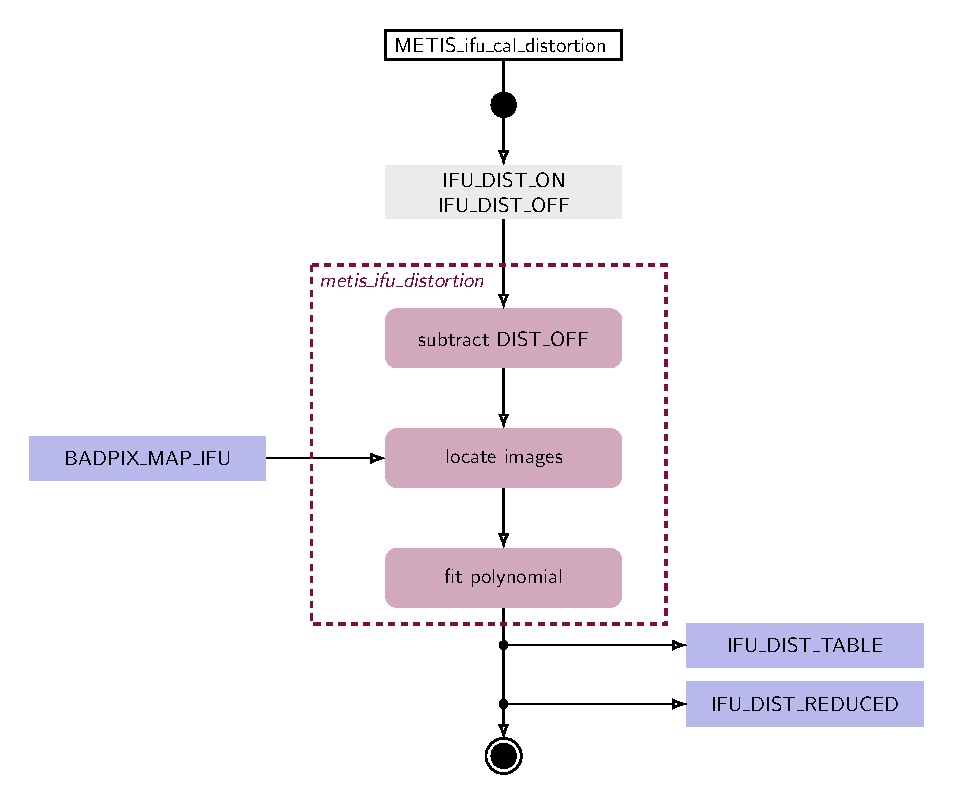
\includegraphics[width=0.6\textwidth]{metis_ifu_distortion}
  \caption[Recipe: \REC{metis_ifu_distortion}]{%
    \hyperref[rec:metis_ifu_distortion]{\REC{metis_ifu_distortion}} -- IFU distortion calibration}
  \label{fig:metis_ifu_distortion}
\end{figure}


\clearpage



%%%%%%%%%%%%%%%%%%%%%%%%%%%%%%%%%%%%%%%%%%%%%%%%%%%%%%%%%%%%%%%%%%%%%%%%%%%%%%%%

%%% Local Variables:
%%% TeX-master: "METIS_DRLD"
%%% End:
